This chapter provides information about optics and microscopy concepts in this work. The first part is dedicated to the basic set of concepts and properties from optics that are necessary for light microscopy; the second one describes the structure of the optical microscope, along with its uses and implications on the acquired images. Plenty of image degradation is due to the system acquisition process; in fact, defocus is a natural occurrence in optics, mainly caused by adjustments of the optical system.


\section{Relevant elements of optics}

The definition of the spectroscopy procedure consists on the interaction between electromagnetic radiation and the matter \cite{gauglitz2006handbook}. This concept can be extended to microscopy, which deals with the range of the electromagnetic spectrum of wavelength between 400 and 700 nanometers, i.e. visible light,  to create visual representations of the objects
\cite{bell2009introduction}. Light microscopy is inherently related to optics, and some concepts of the field are directly related to the blurring process; therefore, it is meaningfully important to elucidate them.

\subsection{Dual Nature of Light}

The light was described in different ways according to different geniuses. Isaac Newton (1642-1727) proposed that light had a corpuscular nature, due to the trajectory in which light appeared to travel in a uniform medium in his experiments; Christiaan Huygens (1629-1695) stated in his works that light was traveling in a ``wave-like'' way and apparently could explain some optical principles such as the interference phenomena \cite{fowles1989introduction}. 

The corpuscular approach for explaining the behavior of light was accepted during the 17th and 18th centuries since Newton played a central role in science in that era. The development of electricity and magnetism as solid fields of research and theoretical representations of natural phenomena was happening concomitantly with optics. Michael Faraday (1791-1867) connected magnetism and light for the first time with his studies on light polarization in magnetic field immersed materials. Later, James Clerk Maxwell (1831-1879) established a complete relation between optics and electromagnetism by defining the displacement current density - a relation that involves the polarization of a medium, the intensity of electric fields and the electric permittivity of vacuum - and writing its differential equations \cite{zilio2009optica}.

Light as an electromagnetic wave is therefore composed of the two vectors and propagates in some particular coordinate direction upon a metric space, e.g. the $\mathit{x}$ coordinate on a three-dimensional Euclidean space. Hence, it is possible to treat light as a wave or particle, according to the application or needs. Light microscopy deals with light as a wave and its related phenomena such as reflection, refraction, interference and diffraction, which will be presented on the following subsections and are useful for a deeper understanding of this work. Posterior studies of Max Planck (1858-1947), Albert Einstein (1879-1955) and Niels Bohr (1885-1962) \cite{fowles1989introduction} linked the prior discoveries with the quantum theory, and therefore differ from this research's scope. Maxwell enunciated that there were two different vectors which could cause a state of disturbance in the space while dealing with electric charges; those consist of the electric vector $\mathit{\mathbf{E}}$ and the magnetic induction vector $\mathit{\mathbf{H}}$. Together, they construct the electromagnetic field \cite{born1999principles}, as shown in \autoref{fig:electromagnetic_wave}.

\begin{figure}[htb]
	\centering
	\caption{\label{fig:electromagnetic_wave} 
		Composition of the electromagnetic wave. The red and the blue curves represent the electric (\textbf{E}) and induction (\textbf{H}) vectorial quantities, respectively.}
	\begin{center}
	    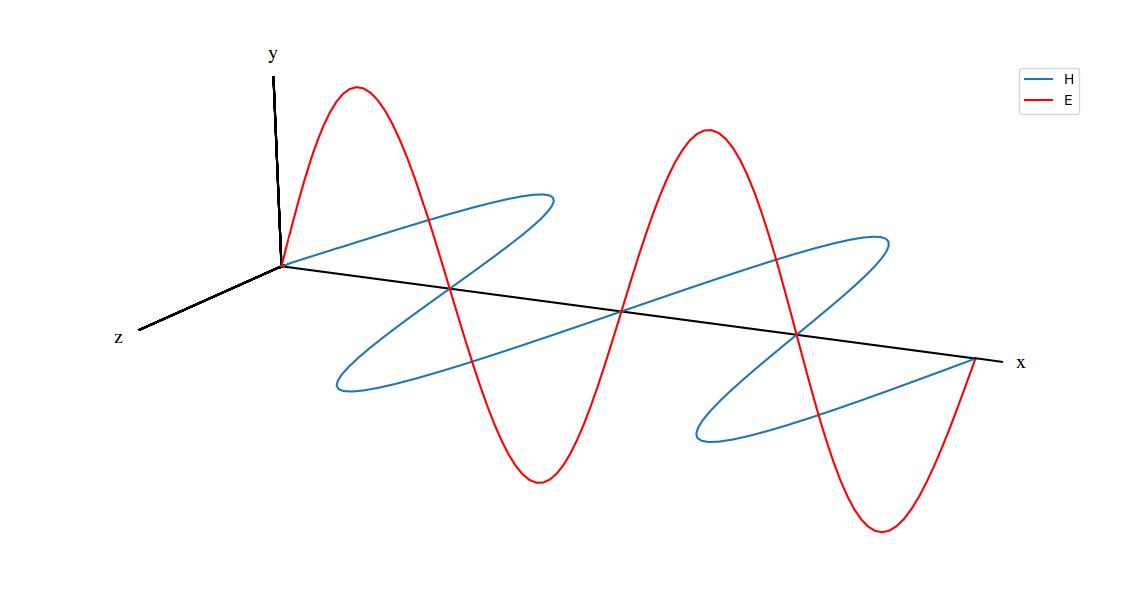
\includegraphics[scale=0.3]
			{images/fig2.png}
	\end{center}
	\centering
	\fautor
\end{figure}

\subsection{Light Wave Properties and Phenomena}

The light waves can be represented by a ray, i.e. a single oriented line which shows the direction of propagation; several waves that propagate in nearly the same direction can be named as a beam \cite{halliday2013fundamentals}. 

% These two models of the real light are important and useful representations within the boundaries of visible light, and allow easier explanations of light properties.

Some relevant properties of waves are explained here according to \citeonline{tipler2007physics}. The frequency ($f$) is the number of cycles per unit of time, or the reciprocal of the time that a periodic wave takes to execute a complete cycle of oscillatory motion $T$, given by $f = T^{-1}$. The Amplitude is the maximum displacement from the equilibrium position, where the wave peak reaches its highest value. Finally, the Phase is a point in time on the cycle of a wave propagation, quantified in degrees.

When rays or beams of light reach surfaces during its propagation, there are four prominent phenomena to consider: reflection, refraction, interference and diffraction. The incident ray of light suffers a split procedure when it reaches a frontier between two homogeneous media. One of the resulting rays reflects within the initial medium and the other one propagates inside the other medium; the first phenomenon is denominated \emph{reflection} and the second, \emph{refraction} \cite{born1999principles}. The speed of light depends on the medium in which it propagates. The \emph{refractive index} is a number that quantifies the speed of light in a particular medium in relation to the speed of light in vacuum, and can be described by

\begin{equation}
    \label{eqn:refractive_index}
       n = \frac{c}{v},
\end{equation}

\noindent where $\mathit{c}$ is the speed of light in vacuum and $\mathit{v}$ is the speed of light in the medium. According to \citeonline{halliday2013fundamentals}, the reflection law states that the resulting ray propagates within the incidence plane and that the angle of reflection $\mathit{\theta^{'}_{1}}$ equals the $\mathit{\theta_{1}}$ angle of incidence; comparably, the refraction law states the same about the incidence plane and relates the incidence $\mathit{\theta_{1}}$ and refraction $\mathit{\theta_{2}}$ angles by Snell's law, given by

\begin{equation}
    \label{eqn:snells_law}
       n_{2}\sin{\theta_{2}} = n_{1}\sin{\theta_{1}},
\end{equation}

\noindent where $\mathit{n_{1}}$ and $\mathit{n_{2}}$ are the refractive indices of the media. This framework consists of an approximation and may be considered ideal for didactic purposes. The process that happens in the real situations may involve non-homogeneous media, opaque or translucent media (which blocks the propagation of light or randomly changes the direction of the rays, respectively), and those concepts are relevant to the imaging procedures, e.g. microscopy. \autoref{fig:beam_split} depicts the real-world phenomenon and its ideal representation.

\begin{figure}[htb]
	\centering
	\caption{\label{fig:beam_split} 
	    (a) Example of a beam of light that reflects and refracts when touching the frontier between air and water. (b) Representation of the process with rays.}
	\begin{center}
	    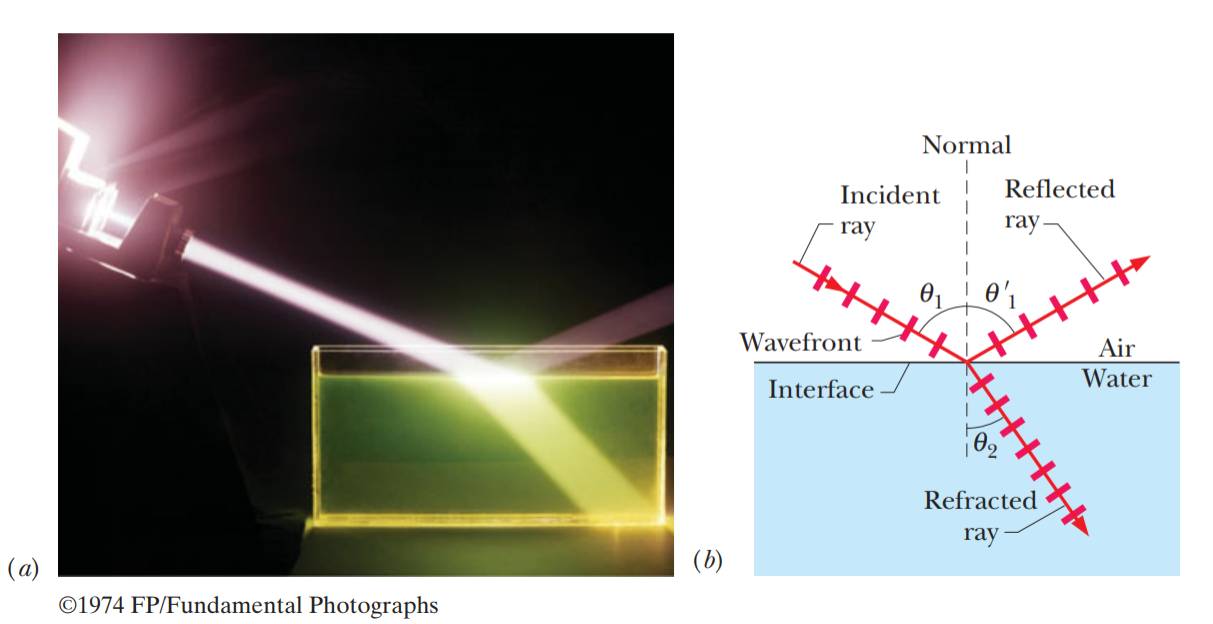
\includegraphics[scale=0.3]{images/fig3.png}
	\end{center}
	\centering
    \fdireta{halliday2013fundamentals}
\end{figure}

When two or more waves of similar or equal frequency superpose in space and form a different intensity pattern, the \emph{interference} of the waves occurred \cite{tipler2008physics}. Mathematically, when interference is observed with light waves, it consists on a vector addition of the electromagnetic fields \cite{zilio2009optica}.
If the interfering waves are in phase, i.e. the difference between the same positions within the wave cycles of the two waves is zero. This process is called \emph{constructive}, which yields a larger amplitude to the new wave. Similarly, if the interfering waves are not in phase, then the process is named \emph{destructive} and yield smaller or null amplitudes to the new wave \cite{tipler2007physics}. Both types of interference are show in \autoref{fig:interference}.

\begin{figure}[htb]
	\centering
	\caption{\label{fig:interference} 
	    (a) Constructive interference and (b) destructive interference.}
	\begin{center}
	    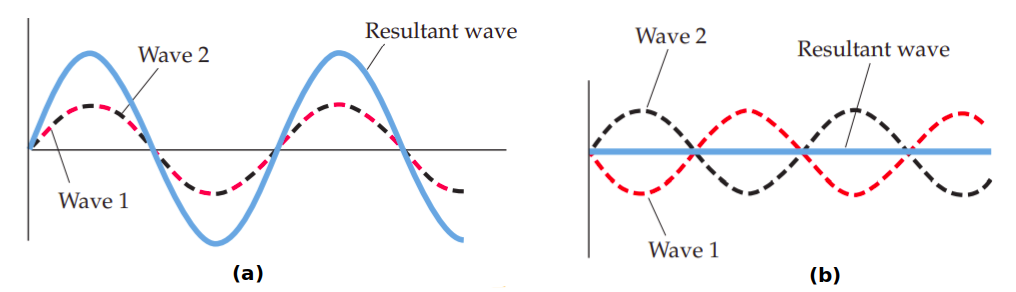
\includegraphics[width=\textwidth,height=4cm, trim=1 1 1 1,clip]{images/interference.png}
	\end{center}
	\centering
    \fadaptada{tipler2007physics}
\end{figure}

The wave theory of light also contains another important property for the real processes: the \emph{diffraction}, a phenomenon that was discovered by Francesco Maria Grimaldi (1618-1663) and consists of the distortion in a wavefront which focuses on obstacles such as apertures on an object, spheres, disks, or anything with similar dimension to the wavelength of the focusing light \cite{zilio2009optica}. The wavefront deviates and scatters after propagating through the obstacle and transforms itself into circular or spherical waves; this is a relevant property that distinguishes a wave from a particle, since the latter would either propagate without any change in its trajectory or would be blocked by the obstacle \cite{tipler2007physics}. When a beam of light reaches an opaque object, the waves suffer changes in their direction of propagation, which can be predicted by the fact that all the points in each wavefront (points of identical phase on waves) generate a new wave, as stated by Huygens \cite{fowles1989introduction}. As described by the Huygens principle, each point of the wavefront acts as a source and creates secondary waves which scatter in every direction; each of the new wavefronts is generated by the interference of an infinite number of sources of waves \cite{zilio2009optica}. The scheme in \autoref{fig:diffraction} illustrates the diffraction phenomenon with an arbitrary obstacle and a small source of waves.

\begin{figure}[htbp]
	\centering
	\caption{\label{fig:diffraction} Diffraction scheme of a wavefront.}
	\begin{center}
	    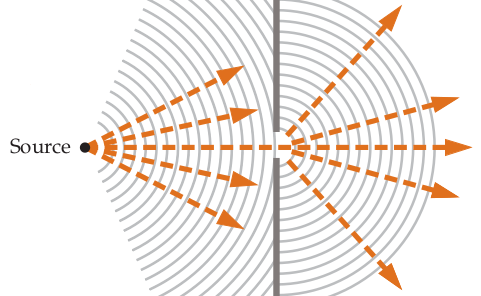
\includegraphics[scale=1.9]{images/diffraction.png}
	\end{center}
	\centering
    \fdireta{tipler2007physics}
\end{figure}

Diffraction is a phenomenon that always happens as waves pass through apertures, but its magnitude depends on the relative proportions between the aperture size and the wavelength: when the latter is large in comparison to the former, the diffraction effects are large and, likewise, a relatively small wavelength yields smaller effects \cite{tipler2007physics}. As stated by \citeonline{zilio2009optica}, there are two common types of diffraction:

\begin{itemize}
    \item \emph{Fresnel Diffraction}: also named near-field diffraction, it occurs when a cylindrical wavefront (the curvature cannot be neglected) passes through an obstacle and diffracts in the near-field, i.e. short distances relative to the path of the diffracted waves' propagation. However, the observation distance is usually finite. It results in different sizes and shapes for the diffraction patterns;
    
    \item \emph{Fraunhofer Diffraction}: also named far-field diffraction, it occurs when planar waves (the curvature of the wavefront may be neglected) pass through an obstacle in the far-field, i.e. large distances relative to the path of the diffracted waves' propagation. Practically, the observation distance is infinite. It results in different sizes for observed aperture images.
    
\end{itemize}

\subsection{Illumination Qualities}

The propagating waves, rays or beams of light that illuminate the object in imaging systems carry some attributes which depend on the source and the desired result. \autoref{fig:illumination_qualities} depicts some relevant qualities of light. 


\begin{figure}[htb]
	\centering
	\caption{\label{fig:illumination_qualities} Comparison between different qualities of an imaging systems' illumination setup.}
	\begin{center}
	    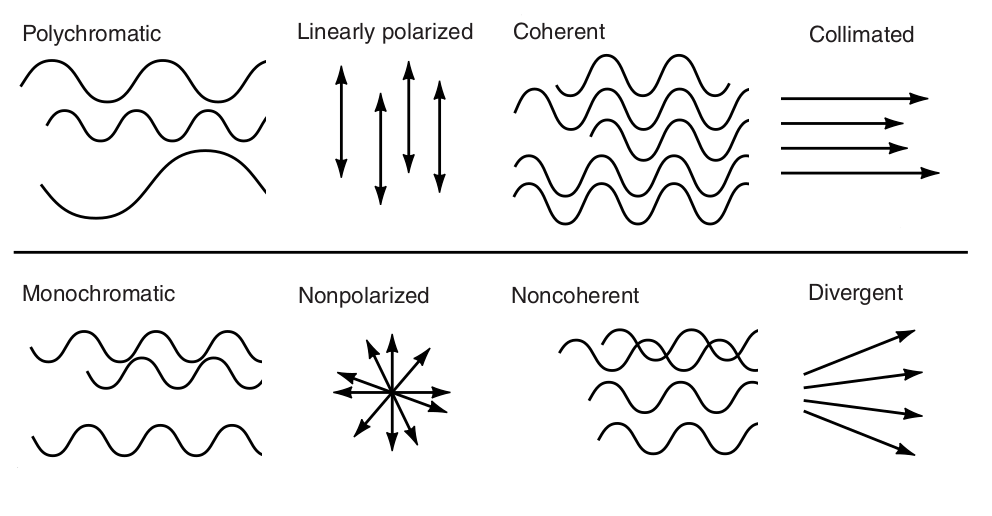
\includegraphics[scale=0.4]{images/light_qualities.png}
	\end{center}
	\centering
    \fadaptada{murphy2012fundamentals}
\end{figure}

Pursuant to \citeonline{murphy2012fundamentals}, the attributes in \autoref{fig:illumination_qualities} 
refer to color, polarization, coherence and direction. Every ray in a \emph{monochromatic} beam has the same wavelength, i.e. the same color, and similarly a \emph{polychromatic} beam consists of a mixture of rays with different wavelengths. The polarization relates to the vibration in the electric vector of light as an electromagnetic wave which may occur in parallel planes (\emph{polarized light}) or not (\emph{nonpolarized light}). The coherence is the relationship between the phase of each wave of a given wavelength: if the phase is the same for all waves, as in a laser beam, the light is named \emph{coherent}, otherwise it is said that the illumination is \emph{noncoherent} or \emph{incoherent}, as in bright-field microscopes. Finally, the waves may propagate in parallel trajectories, i.e. be \emph{collimated}, or may diverge or converge to some point.

\subsection{Properties of the Spherical Lenses}

As stated by \citeonline{halliday2013fundamentals}, \emph{lenses} are objects consisting of a transparent material, with a certain refractive index, that are made of two spherical surfaces on which light propagates and suffers refraction. They are used in optical systems due to their capacity to create images as long as their refractive index is not equal to that of the medium. Yet, in agreement with \citeonline{halliday2013fundamentals}, some concepts related to lenses are important in our context and will be shown below. \autoref{fig:spherical_lens} illustrates an arbitrary spherical lens, with principal elements from geometric optics that relate to lenses and its consequent imaging properties.

\begin{figure}[htb]
	\centering
	\caption{\label{fig:spherical_lens} Arbitrary scheme of the optical properties of a spherical lens: radii of curvature ($r_{1}$, $r_{2}$), centers of curvature ($C_{1}$, $C_{2}$), focal points ($F_{1}$, $F_{2}$) and focal length ($f$).}
	\begin{center}
	    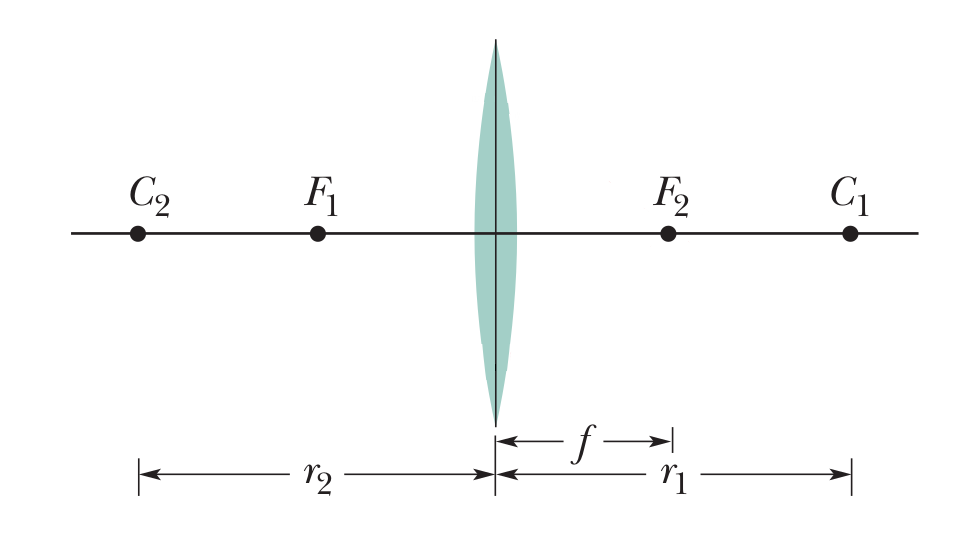
\includegraphics[scale=0.4]{images/fig4.png}
	\end{center}
	\centering
    \fadaptada{halliday2013fundamentals}
\end{figure}

Some properties of the spherical lenses directly influence the image formation process and, consequently, the resulting image quality. The \emph{numerical aperture} (NA), as reported by \citeonline{murphy2012fundamentals}, is a measurement in terms of angles that shows how much light the lenses can capture, and it is given by

\begin{equation}
    \label{eqn:numerical_aperture}
    NA = n \sin{\theta},
\end{equation}

\noindent where $\theta$ is the half angle of the cone of specimen light accepted by the objective lens and $n$ is the refractive index between the lens and the specimen. There are optical flaws in lenses that hinder a proper image formation. Those are named \emph{aberrations} \cite{lawlor2019introduction}, and the most relevant types in the scope of this project are the \emph{spherical aberrations}. According to \citeonline{murphy2012fundamentals}, the spherical aberrations occur when there is a difference in the focal point of incident parallel rays at central and peripheral locations of a spherical lens' surface, which yields a blurred image of either a point source of light or an extended object. It is possible to correct a spherical aberration by changing the shape of the refracting surface, i.e. changing the radius of curvature for the lenses in order to adjust the focal point to one particular distance \cite{smith1988optics}. The illustration in \autoref{fig:spherical_aberrations} represents the spherical aberration for a point source of light, where it is possible to see the difference between incident rays in the borders and in the inner regions of the lens. The resulting image is, in this case, a set of concentric circles around a point.

\begin{figure}[htb]
	\centering
	\caption{\label{fig:spherical_aberrations} Arbitrary example of the spherical aberration.}
	\begin{center}
	    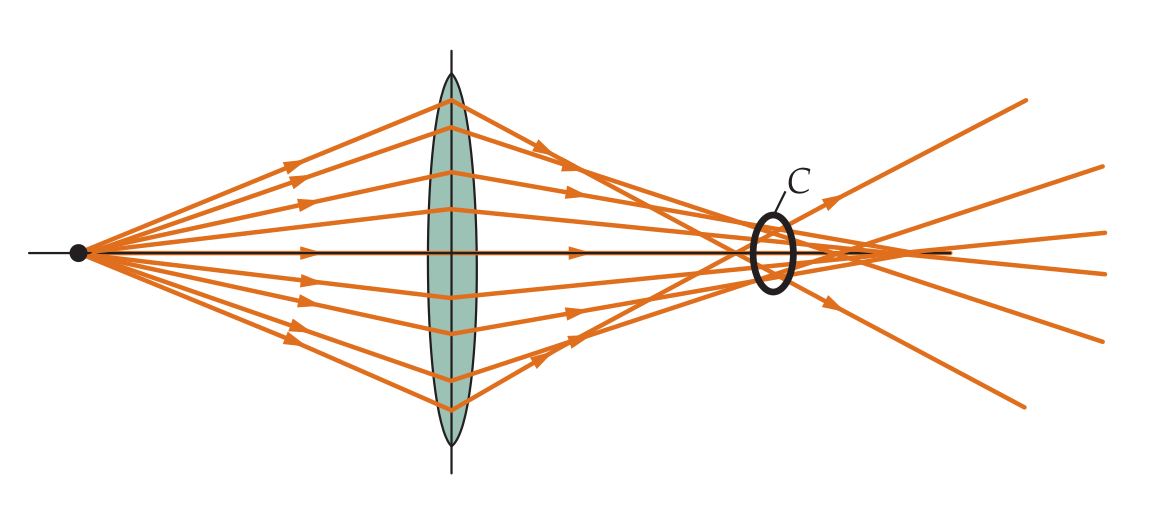
\includegraphics[scale=1.5]{images/spherical_aberration.png}
	\end{center}
	\centering
    \fdireta{tipler2008physics}
\end{figure}

\vspace{-1cm}